The \gls{AURA} platform relies on a hybrid data storage architecture designed to support high-frequency telemetry, versioned \gls{ML} artifacts, relational metadata orchestration, and real-time event logging. The underlying information model is structured across a relational database, a document-based non-relational database, a distributed object storage bucket, and in-memory key-value stores.

\subsubsection{Entities and Relationships}\label{sec:er_diagram}

The relational database layer represents the catalog of physical resources and administrative metadata. There are five main entities defined in the system schema:
\begin{itemize}
    \item \textbf{Devices}: Represents the IoT edge nodes (such as Raspberry Pi or NVIDIA Jetson) that execute inference pipelines and stream telemetry.
    \item \textbf{Models}: Stores metadata for both original PyTorch neural networks and their compiled hardware-specific binaries (e.g., Hailo HEF files).
    \item \textbf{Datasets}: Defines the data catalog and versioned packages used for compiling and fine-tuning edge-compatible models.
    \item \textbf{Scripts}: Contains code for pre- and post-processing inferences (e.g., custom Python routines).
    \item \textbf{Deployments}: An orchestration entity linking a specific device, model, and script to establish a running inference pipeline on an edge node.
\end{itemize}

Below, \autoref{fig:er_diagram} shows the conceptual diagram of relationships between the main entities of the system.

\begin{figure}[H]
    \centering
    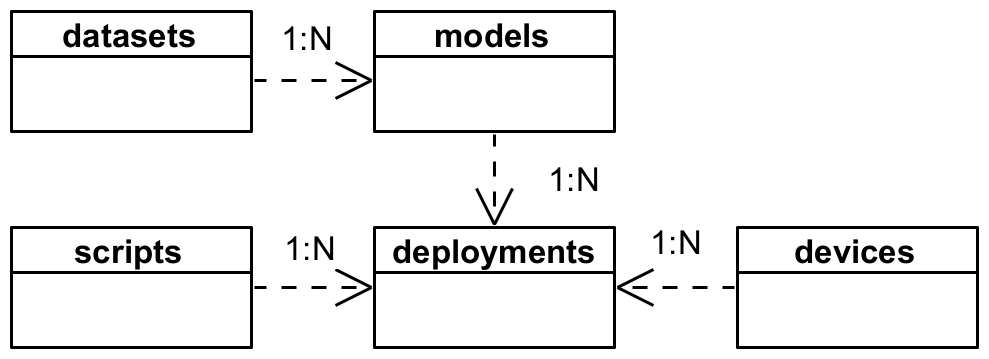
\includegraphics[width=0.8\textwidth]{images/Entities.png}
    \caption{\acrshort{AURA} Entity-Relationship Diagram}
    \label{fig:er_diagram}
\end{figure}

\clearpage

\subsubsection{Data Dictionary (Relational Database)}\label{sec:relational_db}

The database schema contains one table corresponding to each core entity: \texttt{devices}, \texttt{models}, \texttt{datasets}, \texttt{scripts}, and \texttt{deployments}. As shown in \autoref{fig:relational_db}, each table holds descriptive attributes, status values, foreign keys, and unique identifiers. Detailed definitions of each database column, data type constraints, and relationships are provided in \autoref{app:relational_database}.

\begin{figure}[H]
    \centering
    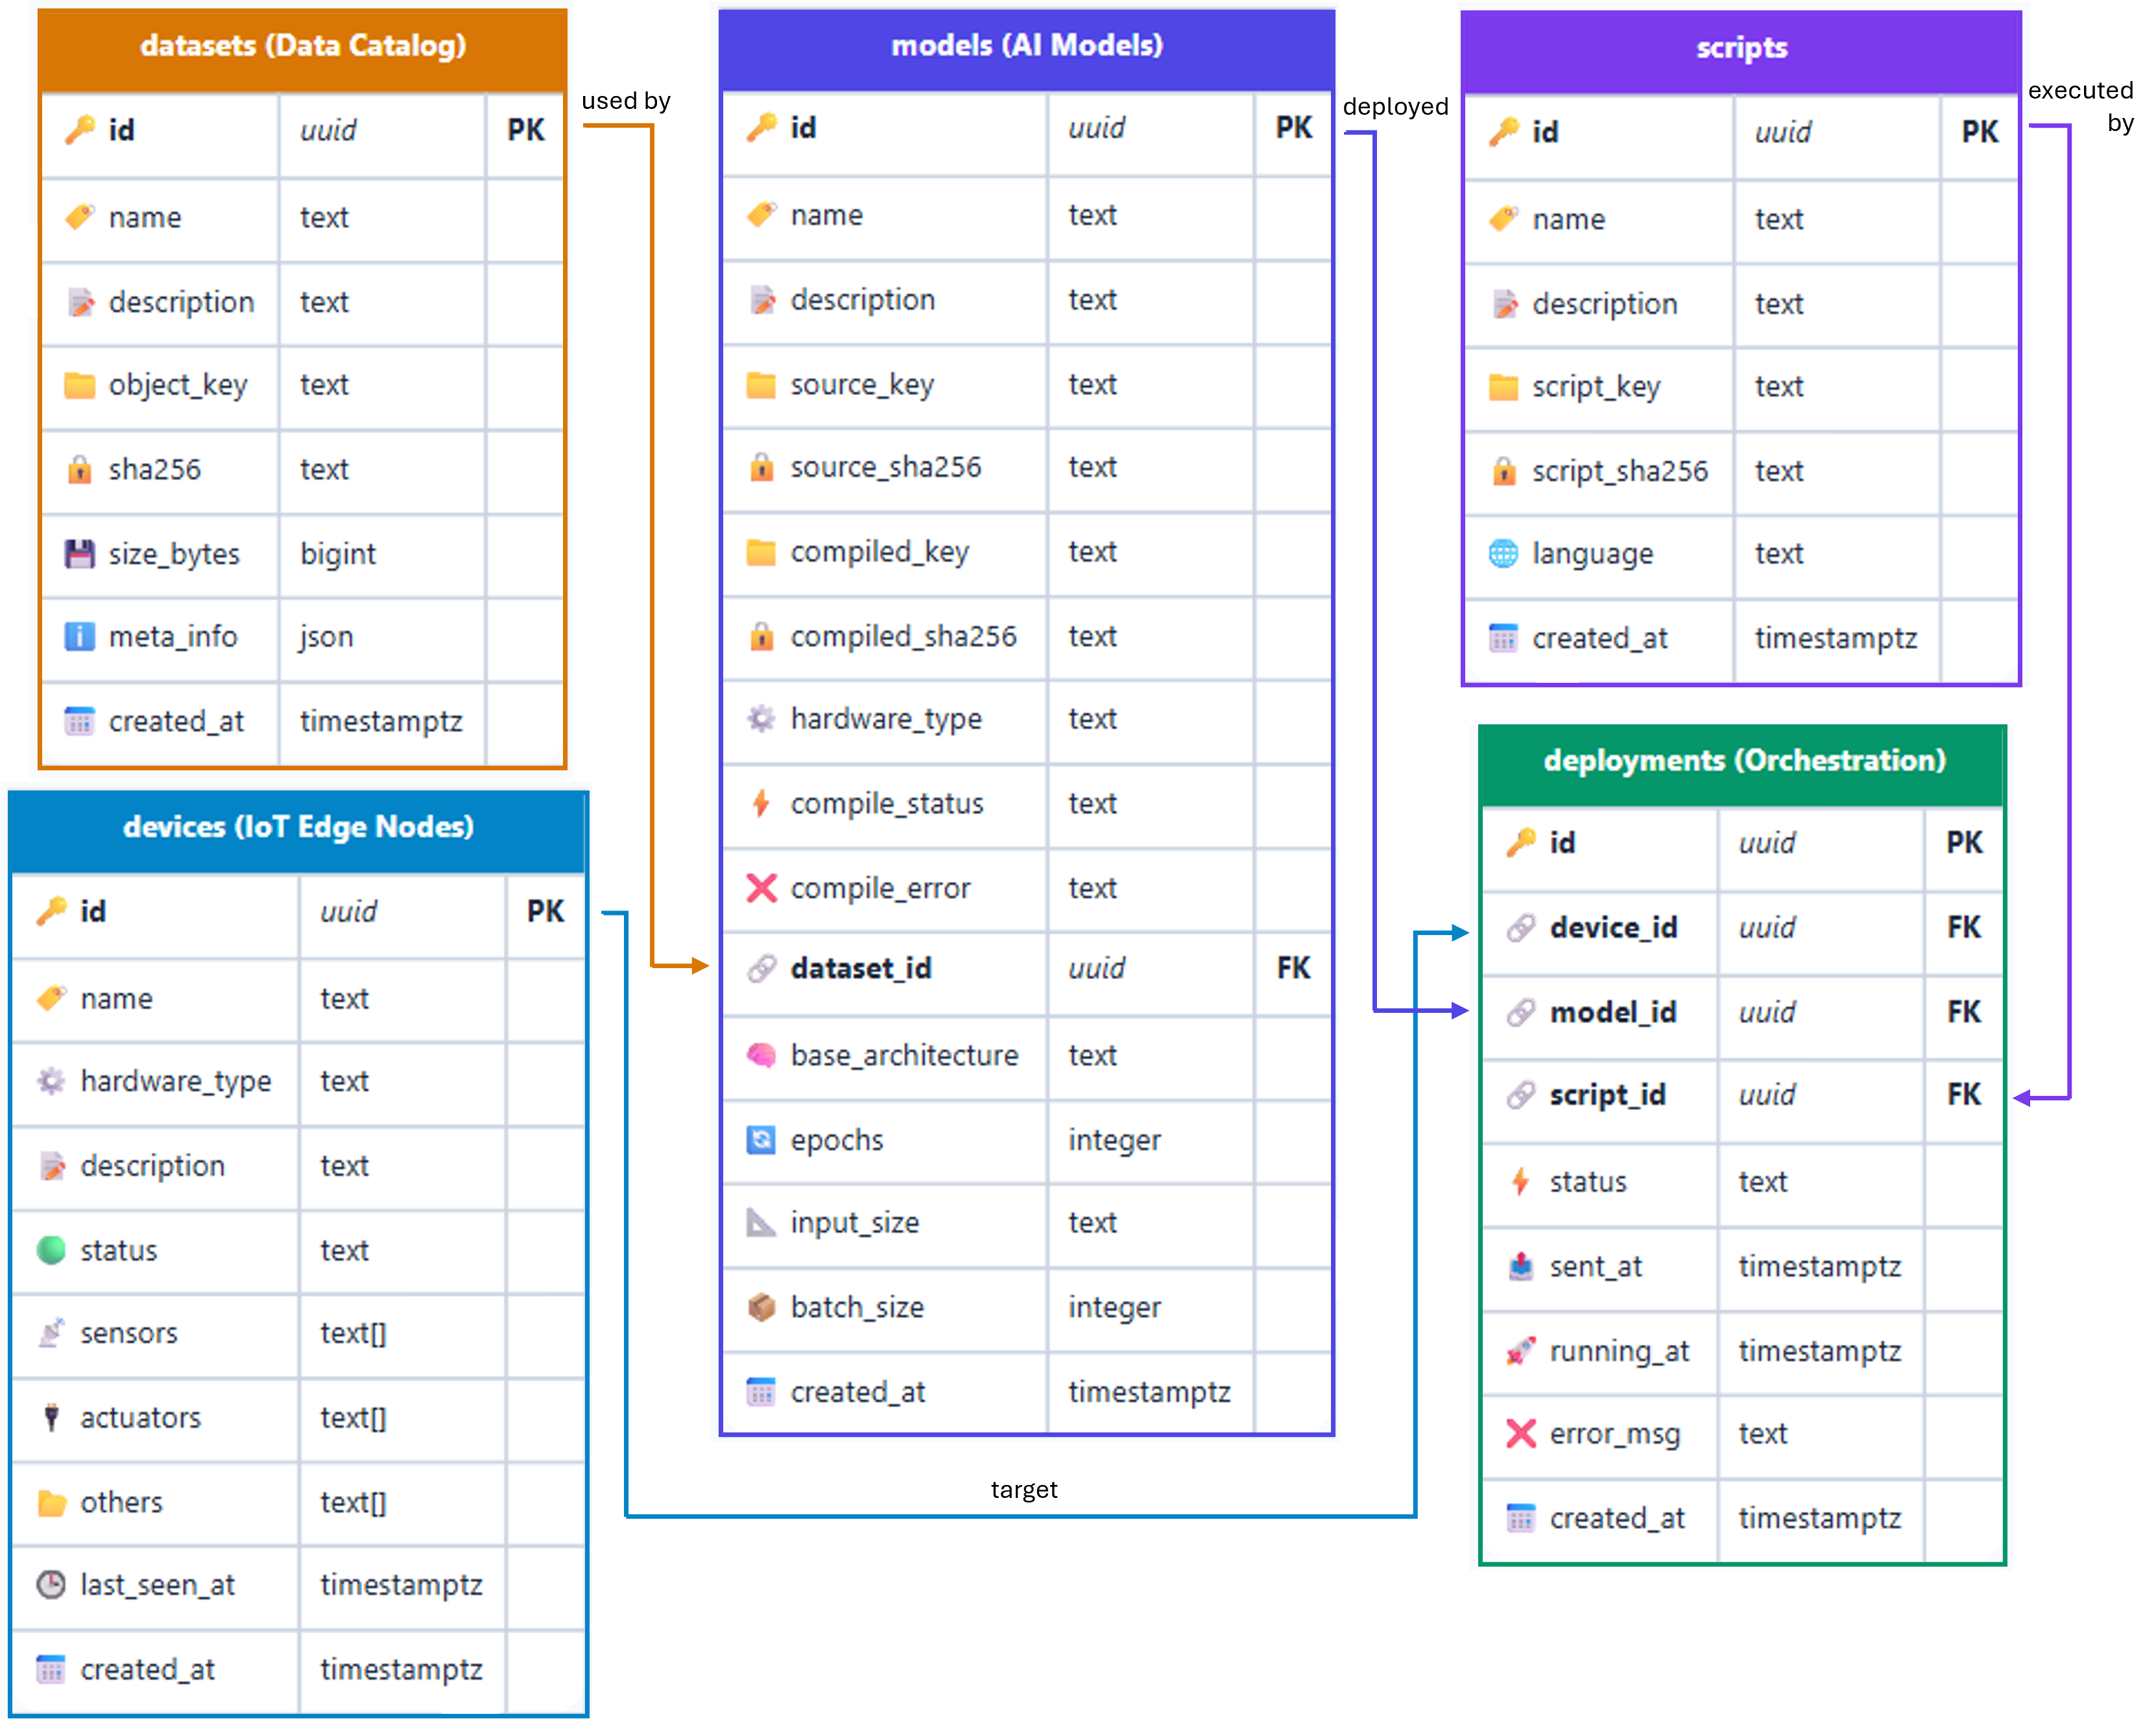
\includegraphics[width=1\textwidth]{images/Relational DB.png}
    \caption{\acrshort{AURA} Data Dictionary Diagram}
    \label{fig:relational_db}
\end{figure}

\subsubsection{Edge Telemetry and Predictions (Non-Relational Database)}\label{sec:non_relational}

High-frequency, volatile, or semi-structured data generated by edge nodes are stored in a non-relational database. This isolates time-series operational telemetry and inference predictions from the transactional relational database. Two main collections are maintained:
\begin{itemize}
    \item \texttt{device\_states}: Holds the latest heartbeat status, active deployments, and geographical coordinates of each edge node.
    \item \texttt{inference\_results}: Appends historical \gls{AI} inferences streamed from edge nodes, storing the timestamp and deployment \gls{ID}.
\end{itemize}

\subsubsection{Object Storage Structure (MinIO)}\label{sec:minio_storage}

Large binary assets are stored in MinIO. To guarantee globally unique object naming, keys are structured around entity \glspl{UUID} as follows:

\begin{itemize}
    \item \textbf{Versioned Datasets}: \texttt{datasets/<dataset\_id>/<version\_id>/<filename>}
    \item \textbf{Original Models (.pt)}: \texttt{models/<model\_id>/source.pt}
    \item \textbf{Compiled Hardware Models (.hef, etc)}: \texttt{compiled/<model\_id>/model.hef}
    \item \textbf{Inference Scripts (.py)}: \texttt{scripts/<script\_id>/script.py}
\end{itemize}

\subsubsection{Task Queue and Log Streaming (Redis)}\label{sec:redis_storage}

An in-memory key-value store (Redis) acts as the central broker for asynchronous task management and real-time event streaming:
\begin{itemize}
    \item \textbf{Asynchronous Task Queue}: It distributes heavy \gls{ML} jobs (such as model compilation and training) to isolated worker processes, preventing resource starvation on the \gls{API} services.
    \item \textbf{Real-Time Log Streaming}: Utilizes Redis Pub/Sub channels and lists to capture and multiplex stdout lines (e.g., training progress console logs) from active worker subprocesses directly to user interfaces.
    \item \textbf{Task Cancellation and Caching}: Caches temporary state flags, such as job cancellation requests and compilation completion statuses, with short-term \gls{TTL} configurations.
\end{itemize}

\subsubsection{Metrics Collection (Prometheus)}\label{sec:prometheus_storage}

Hardware-level metrics are scraped and monitored using a Prometheus exporter running inside the monitoring service. Edge devices periodically stream metrics, which are transformed into Prometheus gauge vectors. Key tracked metrics include:
\begin{itemize}
    \item \texttt{aura\_device\_cpu\_percent}: Measures \gls{CPU} utilization of each edge node.
    \item \texttt{aura\_device\_ram\_percent}: Tracks memory usage percentage.
    \item \texttt{aura\_device\_ram\_used\_mb}: Monitors absolute memory usage in megabytes.
\end{itemize}
All metrics are labeled by \texttt{device\_id} to support granular querying, dashboard rendering, and alerting.

\subsubsection{Communication Commands}\label{sec:commands}

Control and data synchronization commands are exchanged between the cloud control plane and \gls{IoT} Edge devices. Control commands are sent by the Edge Connector Service, while edge nodes report execution events back to dedicated status and event streams.

\begin{itemize}
    \item \textbf{Outgoing Commands}: Cloud-to-device commands are sent using \gls{JSON}-formatted payloads:
    \begin{itemize}
        \item \textbf{Deployment Command}: Sent to trigger the installation of a compiled model and preprocessing script on the edge node.
        \begin{verbatim}
        {
          "command": "deploy",
          "deployment_id": "<uuid>",
          "model_url": "<presigned_s3_url>",
          "model_sha256": "<hash>",
          "script_url": "<presigned_s3_url>",
          "script_sha256": "<hash>"
        }
        \end{verbatim}
    
        \item \textbf{Library Synchronization Command}: Sent to update edge platform libraries dynamically.
        \begin{verbatim}
        {
          "command": "update_libraries",
          "libraries_url": "<presigned_s3_url>",
          "libraries_sha256": "<hash>",
          "directory_sha256": "<hash>"
        }
        \end{verbatim}
    \end{itemize}

    \item \textbf{Incoming Telemetry and Events}: Edge nodes stream telemetry, inference outputs, and operational feedback back to the cloud:
    \begin{itemize}
        \item \textbf{Deployment Events}: Devices publish operational feedback (e.g., \texttt{"deploy\_ack"} or \texttt{"deploy\_failed"}) to confirm the status of deployment instructions.
        \item \textbf{Device Telemetry}: Periodic heartbeats reporting \gls{CPU} usage, memory consumption, active deployment \glspl{ID}, and library directory hashes.
        \item \textbf{Inference Streaming}: Streams real-time prediction results, attaching the deployment \gls{ID} and prediction details.
    \end{itemize}
\end{itemize}